%-*- mode: LaTeX; -*-

\chapter{Discussion}
\label{sec:discussion}
This chapter discusses the results presented in chapter \ref{sec:results}. The chapter is divided into two parts, one part discusses the results of seed growth the other part discusses the results of characterization of the B-doped samples. 

\section{On seed growth}
As shown in section \ref{sec:results:seeds}, carbon face grown seeds did not have complete coverage of cubic SiC on the facet, yet the silicon face grown seeds could reproducibly be grown with complete cubic coverage. As seen in figure \ref{fig:supersaturation}, 2D growth is promoted by high supersaturation. A possible explanation of the results is that the supersaturation for the C-face growth was too low. The examined temperatures, as shown in table \ref{tab:seeds}  range from 1825 to 1925 $^\circ$C, which is a large portion of the parameter space in which the 3C-SiC polytype is stable. Changing the temperature much more during growth is unlikely to result in better 3C-coverage, hence the supersaturation will not be able to be changed much more by altering the temperature. 

From table \ref{tab:seeds} it can be seen that the percentage of the facet covered by 3C-SiC does not show any trend with regards to temperature. The growth time has been adjusted to get similar sample thickness for all samples. In this way it was possible to only vary the supersaturation between samples. This indicates that for the used growth setup it is not possible to change the supersaturation enough to get complete 3C-SiC coverage of the facet. It should however be mentioned that the pressure conditions for growth have not been explored in this work, and that it may be possible to alter the pressure to get more cubic coverage. 

Possible explanations of the difference in 3C-SiC coverage on silicon and carbon face substrates is the spiral growth character. On Si-face the spirals take the form of proper spirals. This gives a structure with steps expanding from the center of the spiral. The C-face spiral takes the form of straight lines extending radially from the center, as seen in figure \ref{fig:carbon_seed1}. The 3C-SiC polytype nucleates on top of the heteroepitaxially grown spirals and grows over the spiral steps. The spiral shape can then be expected to influence how the 3C-SiC is grown. The silicon face spiral may be advantageous for cubic growth, while the carbon face spiral may not be. 

The silicon and carbon faces have different surface energies, which will influence how material grows on it. This may also be a factor in the problem of growing 3C-SiC on the carbon face. From the micrographs of the carbon face seeds it can be seen that cubic growth always occurs at the edge of the facet, i.e. near the graphite spacer. This is consistent with the hypothesis that the surface energy gives rise to the results, since the edge is expected to have a different surface energy compared to somewhere towards the center of the sample. 

%\begin{itemize}
%\item Possible explanation is that the supersaturation is too low (see graph). Supersaturation varies with temperature, we should see a trend when varying temperature. We do not. 
%\item Cannot vary temperature much more, since 3C is only stable in small temperature window. 
%\item Spiral shape is different, maybe this shape is not good for 2D-growth. 
%\item C and Si has different surface energies, which will influence growth. Maybe the C conditions are not compatible with the 3C-growth. 
%\item The surface energy alternative explains why we always see 3C at the edge, never in the center.  
%\end{itemize}

\section{On B-doped samples}
From figure \ref{fig:B_doped_micrographs1} it can clearly be seen that B-doping deteriorates the crystal quality. All doped samples have a larger number of defects compared to the nominally undoped sample. For samples D1 and D4 the number of defects increase with increasing source doping. This is to be expected, since the boron atoms have a different radius compared to both the silicon and carbon atoms it replaces. This size difference will induce strain in the sample and in turn induce defects. From the same figure we can see that sample D6, which was grown with the source material with the highest doping concentration has smoother surface compared to the two other doped samples. This does not follow the trend. In figure \ref{fig:BGe20_micrograph} (b) can be seen that sample D9, grown from the same source material as D6, shows similarly good surface quality. From the absorption measurements of these samples however, it can be inferred that these materials do not have very good quality. As described in chapter \ref{sec:results}, sample D9 does not show any B-CB absorption peak, and D6 does not show the band edge absorption. One possible explanation of this is that the source material does not in fact have the high doping concentration it is thought to have. Another possible explanation is that even though the surface shows a low density of defects, the sample may be of poor crystal quality. This would explain why sample D6 does not show any band edge absorption, which should show even at very low doping concentrations. 

Figure \ref{fig:B_doped_micrographs2} shows the difference in surface morphology of doped samples D1 and D8, which have been grown using the direct and indirect growth method respectively. The fact that they both show similar numbers of surface defects could indicate that both samples have been doped with comparable concentration of boron. As shown earlier a higher concentration of boron will induce more defects on the surface. Figure \ref{fig:abs2} gives a further indication that this hypothesis is valid. In this figure it can be seen that the two samples give similar absorption spectra. Most importantly both spectra show the B-CB peak at around 700 nm. From this it can be concluded that the indirect doping method introduced in this work is able to introduce impurities in a grown sample. The density of introduced impurities is from the results mentioned here thought to be similar, but methods better suited to give impurity concentrations should be used to validate this finding. 

The doped samples D1-D5 and D8 all show band edge absorption and the B-CB absorption peak, but none of the samples shows the VB-B peak, which should be present at around 1700 nm. A possible explanation for this would be that the B-level is near or below the Fermi level, so that the occupancy of the level is too high to show much absorption. The Fermi level can be computed if the doping concentrations are known. It can be assumed that the nitrogen doping concentration is the same in doped samples as in unintentionally doped samples, i.e. the donor concentration is $N_D \approx 10^{16}$ cm$^{-3}$. Assuming that the B-doped samples are of p-type, i.e. $p>>n$, the neutrality condition is
\begin{equation}
\label{eq:neutrality1}
p = N_A^- - N_D^+.
\end{equation}
Since the nitrogen energy level is shallow, it can be assumed that at room temperature all donor atoms are ionized. This gives that $N_D^+ =N_D$. Under the Boltzmann approximation the hole density is
\begin{equation}
\label{eq:p}
p \approx N_Ve^{-E_F/kT},
\end{equation}
were $N_V$ is the valence band density of states, and is given by
\begin{equation}
\label{eq:nv}
N_V = 2\left(\frac{kTm_{d,h}}{2\pi \hbar^2}\right)^{3/2},
\end{equation}
where $m_{d,h}$ is the density of states hole mass. The number of ionized acceptor atoms is governed by the temperature and the Fermi levels distance from the acceptor level. 
\begin{equation}
\label{eq:ionized}
N_A^- = \frac{N_A}{1+2e^{\frac{E_A-E_F}{kT}}}.
\end{equation}
From equations \ref{eq:p}-\ref{eq:ionized} the neutrality condition \ref{eq:neutrality1} can be rewritten as
\begin{equation}
\label{eq:neutrality2}
N_Ve^{-E_F/kT}+2N_Ve^{(E_A-2E_F)/kT}+2N_De^{(E_A-E_F)/kT} - N_A + N_D = 0.
\end{equation}
By using the values $E_A = 0.735$ meV, $m_{d,h} = 0.6\times m_0$ and $T = 300$ K, equation \ref{eq:neutrality2} gives the plot in figure \ref{fig:N_A}, where the graphs represent $N_A$ concentrations of $10^{17}, 10^{18}$ and $10^{19}$ cm$^{-3}$ respectively. It can be seen that for the high est concentration the Fermi level is around 0.57 eV and the highest acceptor concentration gives a Fermi level around 0.70 eV, which is close to the acceptor energy level. From this it can be concluded that for doped samples grown with source impurity concentrations of $10^{18}$ to $10^{19}$ cm$^{-3}$, the Fermi level is below the acceptor energy level, but that there is a significant number of states occupied. This may contribute to the fact that there is no VB-B peak visible in the absorption spectra. 

\begin{figure}[H]
\begin{center}
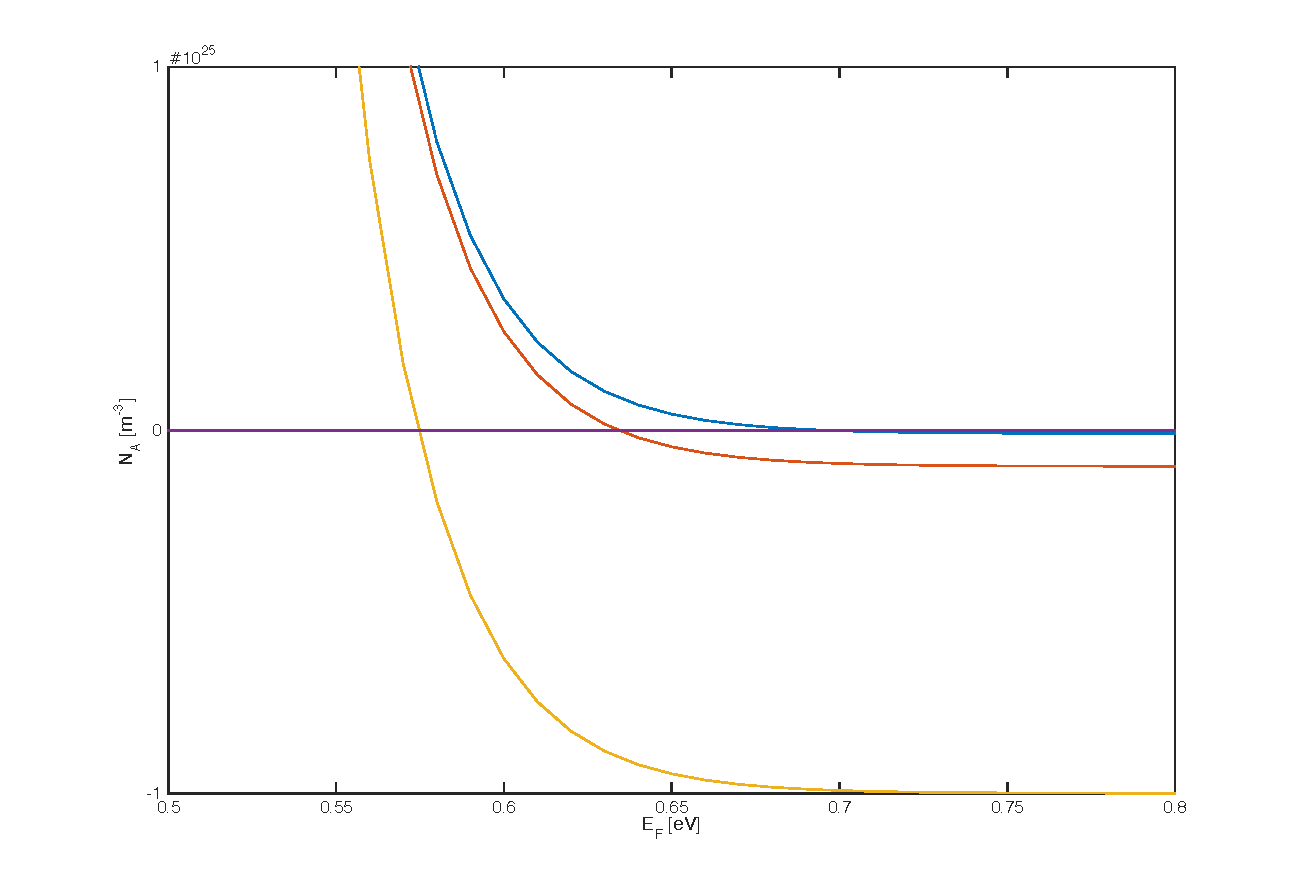
\includegraphics[scale=0.6]{N_A.pdf}
\caption{Computed values of LHS in equation \ref{eq:neutrality2}, plotted against the Fermi level. The three graphs show acceptor concentrations of $10^{17}$, $10^{18}$ and $10^{19}$ cm$^{-3}$. 
\label{fig:N_A}}
\end{center}
\end{figure}


\emph{Outline for PL-discussion}

\begin{itemize}
%\item Surface quality deteriorates with higher doping. Probably due to atomic size difference between B and Si or C. 
%\item However highest doping samples give good surface
%\item Absorption shows no band edge absorption for highest doping samples. This would indicate that the samples are not cubic, or that they have a high density of internal defects.  
%\item[*] Comparing figure with indirect doping with undoped we see a difference in quality. Shows that indirect method gives some result. 
%\item[*] Also the absorption on indirect samples show boron. Shows that indirect method works. The color of the samples would indicate that the doping concentration is lower than in direct growth, for the same source. 
%\item [*] Lowest absorption peak not visible in any B-doped samples. May be due to Fermi level above level [Not so, show calculations]. May be that occupancy too high so only small peak. Crystal quality may make it invisible. 
\item[PL] No luminescence from doped cubic. Would suggest that B-level is non-radiative. Should still show gap luminescence. Maybe crystal quality too poor. 
\item[PL] Al luminescence from one doped cubic sample, shows Al inclusions. Possible competition between the impurity types?
\item[PL] High B luminescence from hex inclusion. Why not in cubic? Maybe hexagonal type of B-placement in hex is radiative, but not the cubic placement. 
\item[PL] People have shown B luminescence from 3C before. Why not us? High doping -> many defects -> maybe the defects are non radiative?
\end{itemize}












































